\documentclass[tikz, border=10pt]{standalone}
\usetikzlibrary{shapes.geometric, arrows.meta, positioning, fit, backgrounds}

\begin{document}
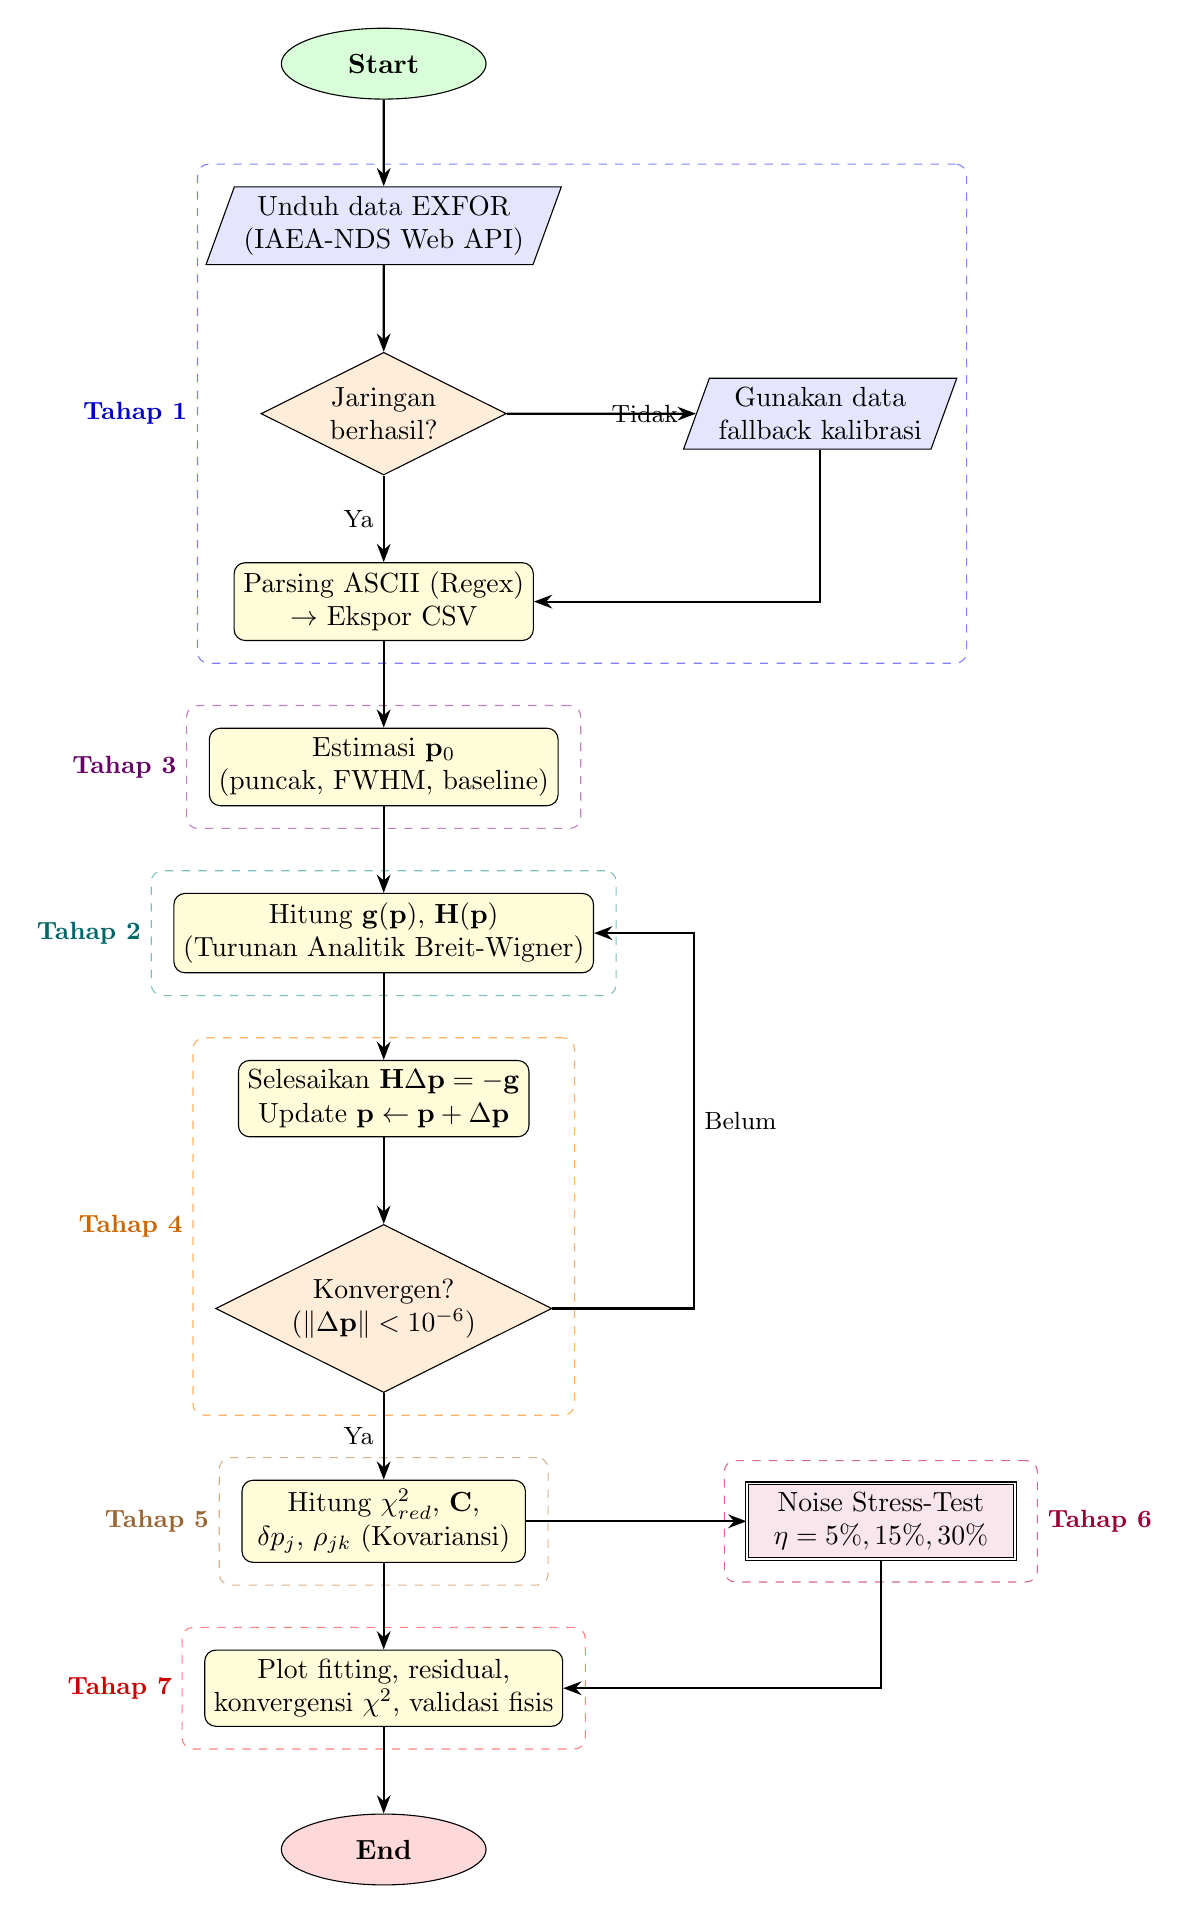
\begin{tikzpicture}[
    node distance=1.1cm and 1.6cm,
    start/.style   = {ellipse, draw, fill=green!15, minimum width=2.6cm, minimum height=0.9cm, font=\bfseries},
    io/.style      = {trapezium, trapezium left angle=70, trapezium right angle=110, draw, fill=blue!10, minimum width=3.2cm, minimum height=0.9cm, align=center},
    process/.style = {rectangle, rounded corners, draw, fill=yellow!15, minimum width=3.6cm, minimum height=0.9cm, align=center},
    decision/.style= {diamond, draw, fill=orange!15, aspect=2, align=center, inner sep=2pt},
    subproc/.style = {rectangle, double, draw, fill=purple!10, minimum width=3.4cm, minimum height=0.9cm, align=center},
    endnode/.style = {ellipse, draw, fill=red!15, minimum width=2.6cm, minimum height=0.9cm, font=\bfseries},
    arrow/.style   = {-Stealth, thick}
]

% --- Tahap 1 ---
\node[start] (start) {Start};
\node[io, below=of start] (fetch) {Unduh data EXFOR\\ (IAEA-NDS Web API)};
\node[decision, below=of fetch] (netok) {Jaringan\\ berhasil?};
\node[io, right=2.4cm of netok] (fallback) {Gunakan data\\ fallback kalibrasi};
\node[process, below=of netok] (parse) {Parsing ASCII (Regex)\\ $\rightarrow$ Ekspor CSV};

% --- Tahap 3 ---
\node[process, below=of parse] (p0) {Estimasi $\mathbf{p}_0$\\ (puncak, FWHM, baseline)};

% --- Tahap 2 & 4 ---
\node[process, below=of p0] (gradhess) {Hitung $\mathbf{g}(\mathbf{p})$, $\mathbf{H}(\mathbf{p})$\\ (Turunan Analitik Breit-Wigner)};
\node[process, below=of gradhess] (solve) {Selesaikan $\mathbf{H}\Delta\mathbf{p}=-\mathbf{g}$\\ Update $\mathbf{p} \leftarrow \mathbf{p}+\Delta\mathbf{p}$};
\node[decision, below=of solve] (conv) {Konvergen?\\ ($\Vert\Delta\mathbf{p}\Vert<10^{-6}$)};

% --- Tahap 5 ---
\node[process, below=of conv] (stats) {Hitung $\chi^2_{red}$, $\mathbf{C}$,\\ $\delta p_j$, $\rho_{jk}$ (Kovariansi)};

% --- Tahap 6 (paralel) ---
\node[subproc, right=2.8cm of stats] (stress) {Noise Stress-Test\\ $\eta=5\%,15\%,30\%$};

% --- Tahap 7 ---
\node[process, below=of stats] (viz) {Plot fitting, residual,\\ konvergensi $\chi^2$, validasi fisis};
\node[endnode, below=of viz] (end) {End};

% --- Arrows ---
\draw[arrow] (start) -- (fetch);
\draw[arrow] (fetch) -- (netok);
\draw[arrow] (netok) -- node[right]{\small Tidak} (fallback);
\draw[arrow] (fallback) |- (parse);
\draw[arrow] (netok) -- node[left]{\small Ya} (parse);
\draw[arrow] (parse) -- (p0);
\draw[arrow] (p0) -- (gradhess);
\draw[arrow] (gradhess) -- (solve);
\draw[arrow] (solve) -- (conv);
\draw[arrow] (conv.east) -- ++(1.8,0) |- node[pos=0.25, right]{\small Belum} (gradhess.east);
\draw[arrow] (conv) -- node[left]{\small Ya} (stats);
\draw[arrow] (stats) -- (viz);
\draw[arrow] (stats.east) -- (stress.west);
\draw[arrow] (stress.south) |- (viz.east);
\draw[arrow] (viz) -- (end);

% --- Pengelompokan visual per tahap ---
\begin{scope}[on background layer]
\node[fit=(fetch)(netok)(fallback)(parse), draw=blue!50, dashed, rounded corners, inner sep=8pt, label={[font=\small\bfseries, text=blue!80!black]left:Tahap 1}] {};
\node[fit=(p0), draw=violet!50, dashed, rounded corners, inner sep=8pt, label={[font=\small\bfseries, text=violet!80!black]left:Tahap 3}] {};
\node[fit=(gradhess), draw=teal!50, dashed, rounded corners, inner sep=8pt, label={[font=\small\bfseries, text=teal!80!black]left:Tahap 2}] {};
\node[fit=(solve)(conv), draw=orange!60, dashed, rounded corners, inner sep=8pt, label={[font=\small\bfseries, text=orange!80!black]left:Tahap 4}] {};
\node[fit=(stats), draw=brown!60, dashed, rounded corners, inner sep=8pt, label={[font=\small\bfseries, text=brown!80!black]left:Tahap 5}] {};
\node[fit=(stress), draw=purple!60, dashed, rounded corners, inner sep=8pt, label={[font=\small\bfseries, text=purple!80!black]right:Tahap 6}] {};
\node[fit=(viz), draw=red!50, dashed, rounded corners, inner sep=8pt, label={[font=\small\bfseries, text=red!80!black]left:Tahap 7}] {};
\end{scope}

\end{tikzpicture}
\end{document}

